
In this section we characterize the transducts of `spiralling' sequences.
Proofs omitted in the text can be found in the appendix.


\begin{definition}\label{def:seq}
  For a function $f : \nat \to \nat$ we define the sequence~$\seq{f} \in \str{\two}$
  by 
  \begin{center}
  $\displaystyle \seq{f} = \prod_{i = 0}^{\infty} 1 0^{f(i)} = 1 0^{f(0)} \, 1 0^{f(1)} \, 1 0^{f(2)} \, \cdots\,.
  $\end{center}
  For a sequence $\seq{f}$, we often speak of the $n$-th \emph{block} of $\seq{f}$ 
  to refer to the occurrence of the word $10^{f(n)}$ in $\seq{f}$.
\end{definition}

In the sequel we often write 
$\seq{f(n)]}$ to denote the sequence~$\seq{n \mapsto f(n)}$.
We note that there is a one-to-one correspondence between functions $f : \nat \to \nat$,
and infinite sequences over the alphabet~$\two$ that start with the letter~$1$ and that
contain infinitely many occurrences of the letter~$1$.
Every degree is of the form $\convclass{\seq{f}}$
for some $f : \nat \to \nat$.

The following lemma is concerned with some basic operations on functions
that have no effect on the degree of $\seq{f}$
(multiplication with a constant, and $x$- and $y$-shifts),
and others by which we may go to a lower degree
(taking subsequences, merging blocks).

\begin{lemma}\label{lem:basic}
  Let $f : \nat \to \nat$, and $a,b \in \nat$.
  It holds that:
  \begin{enumerate}
    \item 
      \label{item:lem:basic:mult}
      $\seq{a f(n)} \fstconv \seq{f(n)}$, for $a \gt 0$,
    \item 
      $\seq{f(n + a)} \fstconv \seq{f(n)}$,
      \label{item:lem:basic:xshift}
    \item 
      $\seq{f(n) + a} \fstconv \seq{f(n)}$,
      \label{item:lem:basic:yshift}
    \item 
      $\seq{f(n)} \fstred \seq{f(an)}$, for $a \gt 0$,
      \label{item:lem:basic:sub}
    \item 
      $\seq{f(n)} \fstred \seq{a f(2n) + b f(2n+1)}$.
      \label{item:lem:basic:merge}
  \end{enumerate}
\end{lemma}
\begin{proof}Recall that, for any $g : \nat \to \nat$,
  with the $n$-th \emph{block} of $\seq{g}$ we mean the factor $10^{g(n)}$ of $\seq{g}$.
  \begin{enumerate}
    \item 
      We have $\seq{a f(n)} \fstred_T \seq{f(n)}$ where $T$ is an FST that replaces 
      every factor $0^a$ by~$0$.
      Clearly, the inverse operation is also FST-realisable, so $\seq{f(n)} \fstred \seq{a f(n)}$.
    \item 
      An FST that prepends 
      $\prod_{i = 0}^{a-1} 1 0^{f(i)}$
      to the incoming word
      witnesses $\seq{f(n + a)} \fstred \seq{f(n)}$.
      For the converse direction, let the FST remove the first $a$ blocks from the input.
    \item 
      To see that $\seq{f(n) + a} \fstred \seq{f(n)}$, 
      consider an FST that removes a factor $0^a$ from every block in $\seq{f(n) + a}$.
      Conversely, $\seq{f(n)} \fstred \seq{f(n) + a}$ is witnessed by an FST that appends $0^a$ to every block.
    \item 
      It is clear that the operation of selecting every $a$-th block is realisable by an FST.
    \item 
      By Theorem~\ref{thm:transducts}.
    \qed
  \end{enumerate}
\end{proof}


\begin{definition}\label{def:periodic}
  Let $A$ be a set.
  A function $f : \nat \to A$ 
  is \emph{ultimately periodic}
  if for some integers $n_0 \ge 0$, $p > 0$ we have
  $f(n + p) = f(n)$ for all $n \ge n_0$.
\end{definition}  

\begin{definition}\label{def:spiralling}
  A function $f : \nat \to \nat$ 
  is called \emph{spiralling}
  if 
  \begin{enumerate}
    \item{}\label{def:spiralling:item:i}
      $\lim_{n \to \infty} f(n) = \infty$, and
    \item{}\label{def:spiralling:item:ii} 
      for every $m \ge 1$, the function $n \mapsto f(n) \bmod m$ is ultimately periodic.
  \end{enumerate}
\end{definition}

Functions with the property \ref{def:spiralling:item:ii} in Definition~\ref{def:spiralling}
have been called `ultimately periodic reducible' by Siefkes \cite{sief:1971} (quotation from \cite{seif:mcna:1976}). 
Note that the identity function is spiralling.
Furthermore scalar products, and pointwise sums and products of spiralling functions 
are again spiralling. 
As a consequence also polynomials $a_k n^k + a_{k-1} n^{k-1} + \cdots + a_0$ are spiralling.

In the remainder of this section, we will characterise the transducts $\sigma$ of $\seq{f}$ for spiralling $f$.
We will show that if such a transduct $\sigma$ is not ultimately periodic, 
then it is equivalent to a sequence $\seq{g}$ for a spiralling function $g$, 
and moreover, $g$ can be obtained from $f$ by a `weighted product'.

\begin{lemma}\label{lem:transducts}
  Let $f : \nat \to \nat$ be a spiralling function.
  We have $\seq{f} \fstred \sigma$
  if and only if 
  $\sigma$ is of the form
  \begin{align}
    \sigma = w \cdot \prod_{i = 0}^{\infty} \prod_{j = 0}^{m-1} p_j \, c_j^{\cyc{i}{j}}
    && \text{where} &&
    \cyc{i}{j} = \frac{f(n_0 + m i + j) - a_j}{z} \,,
    \label{eq:double:prod}
  \end{align}
  for some integers $n_0,m,a_j \ge 0$ and $z > 0$, 
  and finite words~$w, p_j, c_j \in \two^*$ $(0 \le j \lt m)$
  such that $\cyc{i}{j} \in \nat$ for all $i \in \nat$ and $j \in \nat_{<m}$.
\end{lemma}

\begin{proof}
  Assume $\seq{f} \fstred \sigma$ and let $T = \tup{Q,q_0,\delta,\lambda}$ be an FST
  that transduces $\seq{f}$ to $\sigma$.
As $f$ is spiralling, 
  there exist $\ell_0, p \in \nat$, $p > 0$ such that 
  $f(n) \equiv f(n+p) \pmod{\zloops{T}}$ for every $n \ge \ell_0$.
  Moreover, as a consequence of $\lim_{n \to \infty} f(n) = \infty$, there exists $\ell_1 \in \nat$ such that 
  $f(n) \ge |Q|$ for every $n \ge \ell_1$.

  For $n \in \nat$, let $q_n \in Q$ be the state that the automaton $T$ is in, before 
  reading the $n$-th occurrence of $1$ in the sequence $\sigma$
  (i.e., the start of the block $1 0^{f(n)}$). 
By the pigeonhole principle there exist $n_0,m \in \nat$
  with $\max \{\ell_0,\ell_1\} < n_0$ and $m > 0$
  such that $m \equiv 0 \pmod{p}$ and $q_{n_0} = q_{n_0+m}$.
Then, for every $i \in \nat$ and $j \in \nat_{<m}$, we have 
  $f(n_0 + mi + j) \ge |Q|$ and 
  $f(n_0 + mi + j) \equiv f(n_0 + j) \pmod{\zloops{t}}$.
  For $j \in \nat_{<m}$, 
  we define $a_j = \min \{f(n_0 + mi + j) \where i \in \nat\}$.
  Note that $a_j \ge |Q|$.
  Then for all $i \in \nat$ and $j \in \nat_{<m}$ we have: 
  $f(n_0 + mi + j) = a_j + \cyc{i}{j} \cdot z$
  where $\cyc{i}{j} = (f(n_0 + mi + j)-a_j) / z$ and $z = \zloops{T}$.
Using Lemma~\ref{lem:pumping} it follows by induction that
  $q_{n_0+n} = q_{n_0+m+n}$ for every $n \in \nat$.
  Hence
  $q_{n_0+j} = q_{n_0+mi+j}$ for every $i \in \nat$ and $j \in \nat_{<m}$.
  Then, again by Lemma~\ref{lem:pumping}, for every $j \in \nat_{<m}$
  there exist words~$p_j,c_j \in \two^*$
  such that 
  $\lambda(q_{n_0+mi+j}, 1 0^{f(n_0 + mi + j)}) 
    = \lambda(q_{n_0+j}, 1 0^{a_j + \cyc{i}{j} \cdot \zloops{T}}) 
    = p_j c_j^{\cyc{i}{j}}$
  for all $i \in \nat$.
  We conclude that 
  \begin{align*}
    \sigma 
    = \prod_{n = 0}^{\infty} \lambda(q_n,10^{f(n)}) 
    = w \cdot \prod_{i = 0}^{\infty} \prod_{j = 0}^{m-1} p_j \, c_j^{\cyc{i}{j}}\,,
  \end{align*}
  where $w = \prod_{n = 0}^{n_0-1} \lambda(q_n,10^{f(n)})$.

  For the other direction, 
  assume $\sigma$ is of the form \eqref{eq:double:prod}
  for some $n_0,m,a_j,z \in \nat$ with $z > 0$, 
  and~$w, p_j, c_j \in \two^*$ $(0 \le j \lt m)$
  such that $\cyc{i}{j} = (f(n_0 + m i + j) - a_j)/z \in \nat$ for all $i \in \nat$ and $j \in \nat_{<m}$.
We define an FST $T$ such that $\seq{f} \fstred_{T} \sigma'$, where 
  \begin{align*}
    \sigma' = \prod_{i = 0}^{\infty} \prod_{j = 0}^{m-1} p_j \, c_j^{\cyc{i}{j}}
\end{align*}
  Define $T = \tup{Q,q_{m-1}^0,\delta,\lambda}$ 
  where $Q = \{q_j^h \where j \in \nat_{<m},\, {-}a_j \le h < z\}$,
  and 
  \begin{align*}
    \pair{\delta}{\lambda}(q_j^h,0) & = \pair{q_j^{h'}}{0^e} && 
    \text{where $e = 1$ and $h' = 0$ if $h + 1 = z$,} \\[-.5ex]
    &&&\text{and $e = 0$ and $h' = h + 1$, otherwise,} \\
\pair{\delta}{\lambda}(q_j^h,1) & = \pair{q_{j'}^{{-}a_{j'}}}{1} && (j' = j+1 \bmod{m}) \,.
  \end{align*}
  For the verification of $\seq{f} \fstred_{T} \sigma'$ 
  we refer to the proof of Lemma~\ref{lem:wprod:FST}
  that contains a more general construction.
  The transduction $\sigma' \fstred \shift{\length{w}}{\sigma}$ 
  is realised by the FST in Figure~\ref{fig:easy}.
  Clearly also $\shift{\length{w}}{\sigma} \fstred \sigma$ holds, and we conclude $\seq{f} \fstred \sigma$.
  \qed
\end{proof}

\begin{figure}[t]
  \begin{center}
    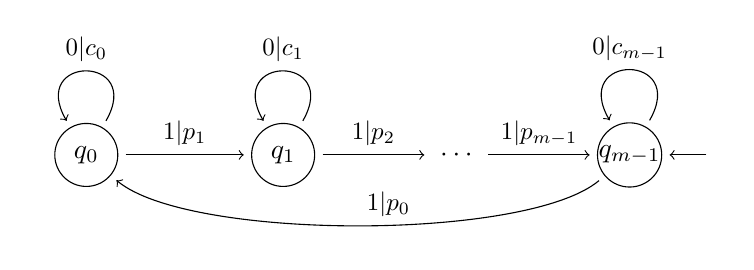
\begin{tikzpicture}[scale=0.9,n/.style={circle,minimum size=8mm,draw,outer sep=1mm,inner sep=0mm}, node distance=25mm, l/.style={scale=.9}]
      \node (q0) [n] {$q_0$};
      \node (q1) [n,right of=q0] {$q_1$};
      \node (q2) [circle,minimum size=8mm,right of=q1,node distance=22mm] {$\cdots$};
      \node (qm-1) [n,right of=q2,,node distance=22mm] {$q_{m-1}$};
      \node (start) [right of=qm-1, node distance=11mm] {};
      \begin{scope}[->]
        \draw (start) -- (qm-1);
        \draw (q0) to[out=60,in=120,looseness=5] node [l,above] {$0|c_0$} (q0);
        \draw (q0) to node [l,above] {$1|p_1$} (q1);
        \draw (q1) to[out=60,in=120,looseness=5] node [l,above] {$0|c_1$} (q1);
        \draw (q1) to[dashed] node [l,above] {$1|p_2$} (q2);
        \draw (q2) to node [l,above] {$1|p_{m-1}$} (qm-1);
        \draw (qm-1) to[out=60,in=120,looseness=5] node [l,above] {$0|c_{m-1}$} (qm-1);
        \draw (qm-1) to[out=-140,in=-40,looseness=.5,pos=.45] node [l,above] {$1|p_0$} (q0);
      \end{scope}
    \end{tikzpicture}
  \end{center}
  \caption{\textit{An FST that transduces $\prod_{i = 0}^{\infty} \prod_{j = 0}^{m-1} 1 \, 0^{\cyc{i}{j}}$
      into $\prod_{i = 0}^{\infty} \prod_{j = 0}^{m-1} p_j \, c_j^{\cyc{i}{j}}$.}}
  \label{fig:easy}
\end{figure}





\begin{example}\label{ex:label}
  We illustrate the influence of both the zero-loops of the automaton 
  as well as the growth of the block lengths of the input sequence,
  on the size~$m$ of the inner product of Lemma~\ref{lem:transducts}.
Consider the FST~$T = \tup{\{q_0,q_1,q_2\},q_0,\delta,\lambda}$ given by 
  \begin{center}
    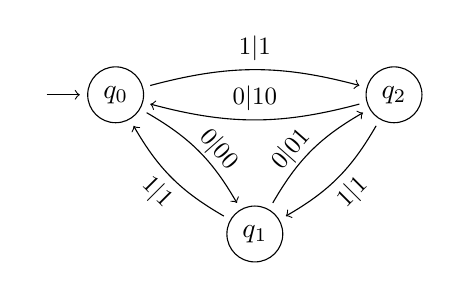
\begin{tikzpicture}[n/.style={circle,minimum size=6mm,draw,outer sep=1mm}, node distance=25mm, l/.style={scale=.9}]
    \node (q0) [n] {$q_0$};
    \node (q1) [n,below right of=q0] {$q_1$};
    \node (q2) [n,above right of=q1] {$q_2$};
    \node (start) [left of=q0, node distance=10mm] {};
    
    \begin{scope}[->]
    \draw (q0) to[bend left=15] node [l,sloped,above,pos=.6,inner sep=.3mm] {$0|00$} (q1);
    \draw (q0) to[bend left=15] node [l,above] {$1|1$} (q2);


    \draw (q1) to[bend left=15] node [l,sloped,below] {$1|1$} (q0);
    \draw (q1) to[bend left=15] node [l,sloped,above,pos=.4,inner sep=.3mm] {$0|01$} (q2);


    \draw (q2) to[bend left=15] node [l,above] {$0|10$} (q0);
    \draw (q2) to[bend left=15] node [l,sloped,below] {$1|1$} (q1);


    \draw (start) -- (q0);
    \end{scope}
    \end{tikzpicture}
  \end{center}
  and the sequence 
  \begin{align*}
    \seq{\floor{\frac{n}{2}}} = 1 1 10 10 10^2 10^2 10^3 10^3 10^4 10^4 \cdots \,,
  \end{align*}
  where $\floor{x} = \max \{ n \in \nat \where n \le x \}$.
We investigate the sequence $r_0 a_0 r_1 a_1 r_2 \cdots$ of states~$r$ of $T$ alternated 
  with letters~$a$ from the input sequence, in such a way that $T$ is in state $r_n$ 
  after having read the word $a_0 a_1 \cdots a_{n-1}$,
  \begin{align*}
\underline{q_0} 1 q_2 1 q_1 1 q_0 0 q_1 1 q_0 0 
    q_1 1 q_0 0 q_1 0 q_2 1 q_1 0 q_2 0 
    \underline{q_0} 1 q_2 0 q_0 0 q_1 0 q_2 1 q_1 0 q_2 0 q_0 0 \cdots
  \end{align*}
  The two underlined occurrences of $q_0$ indicate a repetition of states 
  in combination with a repetition of the block size modulo $\zloops{T} = 3$.
  The number of blocks between these occurrences, forming the repetition, is $m = 6$.
  Actually, following the proof of Lemma~\ref{lem:transducts} precisely, 
  the algorithm would instead select the repetition 
  starting from the second underlined occurrence of $q_0$. 
  The reason is that in general, when reading a block $100\cdots0$,
  only after reading $|Q|$ zeros, we are guaranteed to be in a zero-loop.
  For this FST~$T$, all states are on a zero-loop, 
  and so we enter the loop immediately.
\end{example}

From Lemma~\ref{lem:transducts} it follows that FSTs can only transform 
the length of blocks by linear functions (and merge blocks).
As a consequence, FSTs typically cannot slow down the growth rate of blocks 
in spiralling sequences by more than a linear factor.
This yields the following simple criterion for non-reducibility. 
\begin{lemma}\label{lem:too:fast}
  Let $f,g : \nat \to \nat$ be
  such that $f$ is spiralling, $g$ is not ultimately periodic and $g \in o(f)$, 
  i.e., for every $a \in \nat$ there is $n_0 \in \nat$
  such that for all $n \ge n_0$ it holds that $f(n) \ge a g(n)$.
  Then $\seq{f} \not\fstred \seq{g}$. \end{lemma}
Note that the reverse $\seq{g} \not\fstred \seq{f}$ does \emph{not} follow.
For example, we have $\seq{4^n} \not\fstred \seq{2^n}$, but $\seq{2^n} \fstred \seq{4^n}$.

There can be several ways to factor the transduct~$\sigma$ 
in the statement of Lemma~\ref{lem:transducts},
as shown by the following example.

\begin{example}\label{ex:ambigue}
  Consider the following FST~$T = \tup{\{q_0,q_1\},q_0,\delta,\lambda}$
  \begin{center}
    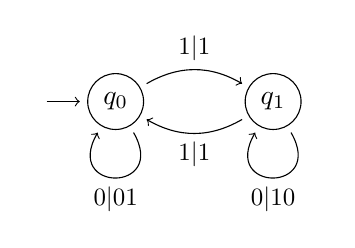
\begin{tikzpicture}[n/.style={circle,minimum size=6mm,draw,outer sep=1mm}, node distance=20mm, l/.style={scale=.9}]
      \node (q0) [n] {$q_0$};
      \node (q1) [n,right of=q0] {$q_1$};
      \node (start) [left of=q0, node distance=10mm] {};
      
      \begin{scope}[->]
      \draw (q0) to[bend left=30] node [l,above] {$1|1$} (q1);
      \draw (q0) to[out=-60,in=-120,looseness=5] node [l,below] {$0|01$} (q0);
  
      \draw (q1) to[bend left=30] node [l,below] {$1|1$} (q0);
      \draw (q1) to[out=-60,in=-120,looseness=5] node [l,below] {$0|10$} (q1);
  
      \draw (start) -- (q0);
      \end{scope}
    \end{tikzpicture}
  \end{center}
  together with the sequence $\seq{n} = 1 10 10^2 10^3 10^4 \cdots$.
  The $T$-transduct of $\seq{n}$ is 
  \begin{align*}
    T(\seq{n}) = 1 \, 1 (01) \, 1 (10)^2 \, 1 (01)^3 \, 1 (10)^4 \, \cdots\,.
  \end{align*}
Using the double product~\eqref{eq:double:prod} of Lemma~\ref{lem:transducts} 
  we have $w = \emptyword$,
  $n_0 = 0$, $m = 2$, $p_0 = p_1 = 1$, $c_0 = 01$, $c_1 = 10$, $a_0 = a_1 = 0$, and $z = \zloops{T} = 1$.
  Thus, $\cyc{i}{j} = 2i + j$.  
Note that $c_1^\omega = p_0 c_0^\omega$, and so we can merge the factors of the inner product, and decrease its size to $m = 1$.
  Then $T(\seq{n}) = 1101 \, 1101 (0101) \, 1101 (0101)^2 \, 1101 (0101)^3 \, \cdots$, that is, 
  in the double product~\eqref{eq:double:prod}, $T(\seq{n})$ can be factored by choosing 
  $m = 1$, $p_0 = 1101$, and $c_0 = 0101$.
\end{example}

Whenever we have the situation $c_j^\omega = p_{j+1}c_{j+1}^\omega$ in the representation~\eqref{eq:double:prod}
for some $j \in \nat_{<m}$ (addition is modulo~$m$), we speak of a `transition ambiguity'.
We will eliminate such ambiguities by merging factors of the inner product, 
as in~Lemma~\ref{lem:merge}.
In general, this merging may involve weighted sums in the exponents. 
The following lemma is folklore, see for instance~\cite{caut:mign:shal:wang:yazd:2003}.
\begin{lemma}\label{lem:folk}If a sequence $\sigma$ is periodic with period lengths $k$ and $\ell$,
  then it is periodic with period length $\gcd(k,\ell)$. \end{lemma}


\begin{lemma}\label{lem:merge}
  Let $u,v,w \in \two^*$ be finite words with $u,w \ne \emptyword$ such that $u^\omega = v w^\omega$.
  Then there exists a word $x \in \two^*$ and $a,b \in \nat$ such that
  $u^m vw^n = vx^{am+bn}$ for all $m,n \in \nat$.  
\end{lemma}
\begin{proof}Let $d = \gcd(|u|,|w|)$, $a = |u|/d$ and $b = |w|/d$.
  Let $x$ be the suffix of~$w$ of length $d$.
  We argue that this choice has the desired property. The sequence $\sigma = u^\omega = v w^\omega$ is periodic with period lengths $|u|$ and $|w|$.
  By Lemma~\ref{lem:folk}
it follows that $\sigma$ is also periodic with period length~$d$.
  Hence $w = x^b$ and 
  for all $m,n \in \nat$, $u^m v w^n$ 
  is a prefix of $\sigma$.
  Likewise $v x^{am + bn}$ is a prefix of~$\sigma = v x^\omega$,
  and both prefixes have the same length:
  $|u^m vw^n| = m|u| + |v| + n|w| = |v| + am|x| + bn|x| = |v x^{am + bn}|$.
  We conclude $u^m vw^n = v x^{am + bn}$.
  \qed
\end{proof}

Our goal is to obtain a simple characterisation of the degrees of the transducts~$\sigma$ 
of spiralling sequences~$\seq{f}$.
To this end, we transform the transduct~$\sigma$ into a sequence~$\sigma'$
by replacing in the double product of Lemma~\ref{lem:transducts}
the displayed occurrence of~$p_j$ by~$1$ and of~$c_j$ by~$0$ 
for every $j \in \nat_{<m}$.
To guarantee that this transformation does not change the degree, 
that is $\sigma' \fstconv \sigma$,
we first have to resolve transition ambiguities.

For the back transformation blocks $10^{\cyc{i}{j}}$ 
have to be replaced by $p_j c_j^{\cyc{i}{j}}$,
an operation that is easily realised by an FST,
see Figure~\ref{fig:easy}.

If the product does not contain transition ambiguities, 
then also the transformation from $\sigma$ into $\sigma'$ 
can be realised by an FST and thus does not change the degree of the sequence, 
hence $\sigma \fstconv \sigma'$.
If there exists $j \in \nat_{<m}$ with
$c_j^\omega = p_{j+1}c_{j+1}^\omega$,
then, by this transformation of $\sigma$ into $\sigma'$, 
one possibly leaves the degree of $\sigma$,
i.e., $\sigma' \fstredstrict \sigma$.
because for large enough~$i\in\nat$, 
an FST cannot recognise where a block~$p_j c_j^{\cyc{i}{j}}$ ends 
and where the next block~$p_{j+1} c_{j+1}^{\cyc{i}{j+1}}$ starts.
This might make it impossible to realise the transformation by an FST,
as then the FST cannot replace $p_{j+1}$ by $1$.


\begin{definition}\label{def:weighted:product}
  A \emph{weight} is a tuple $\tup{a_0,\ldots,a_{k-1},b} \in \rat^{k+1}$ 
  of rational numbers
  such that $a_0,\ldots,a_{k-1} \ge 0$. Given a weight~$\alpha = \tup{a_0,\ldots,a_{k-1},b}$ and a function $f : \nat \to \nat$
  we define
  $\wof{\alpha}{f} \in \rat$ by
  \begin{align*}
    \wof{\alpha}{f} \;=\; a_0 f(0) + a_1 f(1) + \cdots + a_{k-1} f(k-1) + b \,.
  \end{align*}
  The weight~$\alpha$ is called \emph{constant} when $a_j = 0$ for all $j \in \nat_{<k}$.
  For a tuple of weights $\vec{\alpha} = \tup{\alpha_0,\ldots,\alpha_{m-1}}$ 
  we define its \emph{rotation} by $\vec{\alpha}' = \tup{\alpha_1,\ldots ,\alpha_{m-1},\alpha_0}$.
  


  For functions $f : \nat \to \nat$,
  and tuples $\vec{\alpha} = \tup{\alpha_0,\alpha_1,\ldots, \alpha_{m-1}}$ of weights,
  the \emph{weighted product} of $\vec{\alpha}$ and $f$ is a function $\wprod{\vec{\alpha}}{f} : \nat \to \rat$
  that is defined by induction on $n$ through the following scheme of equations: 
  \begin{align*}
    (\wprod{\vec{\alpha}}{f})(0) & = \alpha_0 \cdot f \\
    (\wprod{\vec{\alpha}}{f})(n+1) & = (\wprod{\vec{\alpha}'}{\shift{|\alpha_0|-1}{f}})(n) && (n \in \nat)
  \end{align*}
  where $|\alpha_i|$ is the length of the tuple $\alpha_i$,
  and $\shift{k}{f} $ is the $k$-th shift of $f$.
A weighted product $\wprod{\vec{\alpha}}{f}$ is called \emph{natural} 
  if $(\wprod{\vec{\alpha}}{f})(n) \in \nat$ for all $n \in \nat$. 
\end{definition}

In what follows, all weighted products $\wprod{\vec{\alpha}}{f}$ that we consider are assumed to be natural.

\begin{example}
  Let $f(n) = n$ for all $n \in \nat$, 
  and $\vec{\alpha} = \tup{\alpha_1,\alpha_2}$
  with $\alpha_1 = \tup{1,2,3,4}$, $\alpha_2 = \tup{0,1,1}$.
  Interpreting the functions $f$ and $\wprod{\vec{\alpha}}{f}$ as sequences,
  the computation of $\wprod{\vec{\alpha}}{f}$ can be visualised as follows:
  \begin{center}
    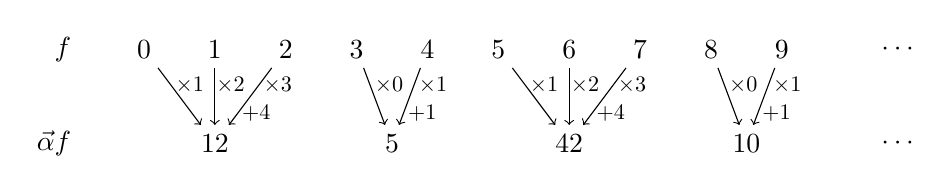
\begin{tikzpicture}
      \node at (-.8cm,0) [anchor=east] {$f$};
      \node at (11*.9cm,0) [anchor=east] {$\cdots$};
      \foreach \i in {0,1,2,3,4,5,6,7,8,9} {
        \node (\i) at (\i*.9cm,0) {\i};
      }
      \node at (-.8cm,-1.2cm) [anchor=east] {$\wprod{\vec{\alpha}}{f}$};
      \node at (11*.9cm,-1.2cm) [anchor=east] {$\cdots$};
      \foreach \i/\x/\v in {0/1/12,1/3.5/5,2/6/42,3/8.5/10} {
        \node (s\i) at (\x*.9cm,-1.2cm) {\v};
      }
      \begin{scope}[inner sep=0,->,nodes={scale=.8}]
      \draw (0) -- node [xshift=3mm,pos=.3] {$\times1$} (s0); 
      \draw (1) -- node [xshift=2.5mm,pos=.3] {$\times2$} (s0); 
      \draw (2) -- node [xshift=3mm,pos=.3] {$\times3$} node [xshift=3mm,pos=.8] {$+4$} (s0); 
      \draw (3) -- node [xshift=3mm,pos=.3] {$\times0$} (s1); 
      \draw (4) -- node [xshift=3mm,pos=.3] {$\times1$} node [xshift=3mm,pos=.8] {$+1$} (s1); 
      \draw (5) -- node [xshift=3mm,pos=.3] {$\times1$} (s2); 
      \draw (6) -- node [xshift=2.5mm,pos=.3] {$\times2$} (s2); 
      \draw (7) -- node [xshift=3mm,pos=.3] {$\times3$} node [xshift=3mm,pos=.8] {$+4$} (s2); 
      \draw (8) -- node [xshift=3mm,pos=.3] {$\times0$} (s3); 
      \draw (9) -- node [xshift=3mm,pos=.3] {$\times1$} node [xshift=3mm,pos=.8] {$+1$} (s3); 
      \end{scope}
    \end{tikzpicture}
  \end{center}
  Thus, for $n = 0,1,2,3\ldots$\,, $(\wprod{\vec{\alpha}}{f})(n)$ takes the values $12,5,42,10,\ldots$\,. 
\end{example}


\begin{lemma}\label{lem:wprod:nth}
  Let $\vec{\alpha}$ be an $m$-tuple of weights ($m > 0$), and let $f : \nat \to \nat$.
  For all $n \in \nat$ we have 
  $(\wprod{\vec{\alpha}}{f})(n) = \wof{\alpha_r}{\shift{t}{f} }$
  where $q,r \in \nat$ with $r < m$ are such that $n = qm + r$,
  and $t = q \cdot \sum_{j = 0}^{m-1}(\length{\alpha_j} - 1) + \sum_{j = 0}^{r-1}(\length{\alpha_j} - 1)$.
\end{lemma}
\begin{proof}
  By induction on $n \in \nat$ we show that, 
  for all $f : \nat \to \nat$, and all $m$-tuples of weights~$\vec{\alpha}$, 
  we have
  \begin{align*}
    (\wprod{\vec{\alpha}}{f})(n) = \wof{\alpha_r}{\shift{t}{f}}
    &&&\text{where $n = qm + r$, and $q,r \in \nat$ with $r < m$,}\\
    &&&\text{and $t = q \cdot \sum_{i = 0}^{m-1}(\length{\alpha_i} - 1) + \sum_{i = 0}^{r-1}(\length{\alpha_i} - 1)$.}
  \end{align*}
  The base case, $n = 0$ follows directly from the definition.
  For the induction step let $\vec{\alpha}$ and $f : \nat \to \nat$ be arbitrary,
  let $n = n' + 1$, $q' = \floor{n'/m}$, and $r' = n' - q'm$.
  We abbreviate $k_i = \length{\alpha_i} - 1$ ($i \in \nat_{<m}$) 
  and $s_\ell = \sum_{i=0}^{\ell-1}$ ($\ell \in \nat_{\le m}$).
  By Definition~\ref{def:weighted:product} and the induction hypothesis we obtain
  \begin{align*}
    (\wprod{\vec{\alpha}}{f})(n) 
    = (\wprod{\vec{\alpha}'}{\shift{k_0}{f}})(n') 
    = \wof{\alpha_{r'+1}}{\shift{t'}{\shift{k_0}{f}}}
  \end{align*}
  with $t' = q' \cdot s_m + s_{r'+1} - k_0$, 
  and where addition in the subscript of $\alpha$ is modulo~$m$.
  We conclude $(\wprod{\vec{\alpha}}{f})(n) = \wof{\alpha_{r}}{\shift{t}{f}}$
  where $n = (q'+1)m$, $r = 0$ and $t = (q'+1) \cdot s_m$ if $r' = m - 1$,
  and $n = q'm + r$, $r = r' + 1$ and $t = q' \cdot s_m + r$ if $r' < m - 1$.
\end{proof}

\begin{lemma}\label{lem:wprod:not:botdeg}
  Let $f : \nat \to \nat$.
  If $\seq{\wprod{\vec{\alpha}}{f}} \not\in \botdeg$, 
  then there exists $i \in \nat_{<\length{\vec{\alpha}}}$ such that $\alpha_i$ is a non-constant weight.
\end{lemma}
\begin{proof}Assume $\alpha_i$ is a constant weight for all $i \in \nat_{<\length{\vec{\alpha}}}$; 
  let $\alpha_i = \tup{0,0,\ldots,0,b_i}$. Then $\wprod{\vec{\alpha}}{f} : \nat \to \nat$ is periodic: for all $n\in\nat$, 
  we have $(\wprod{\vec{\alpha}}{f})(n) = b_i$ where $i \equiv n \pmod{\length{\vec{\alpha}}}$
  and $i \in \nat_{<\length{\alpha}}$. Hence $\seq{\wprod{\vec{\alpha}}{f}} \in \botdeg$.
\end{proof}


We define the operation~$\zip$~\cite{grab:endr:hend:klop:moss:2012} also known as `perfect shuffle'.
 

\begin{definition}\label{def:zip}
  Let $k \in \nat$. 
  For $i \in \nat_{<k}$, 
  let $f_i : \nat \to \nat$ be a function.
  We define the function $\zip_k(f_0,f_1,\ldots,f_{k-1}) : \nat \to \nat$ by 
  \begin{align*}
    \zip_k(f_0,f_1,\ldots,f_{k-1})(kn+i) = f_i(n) && (n \in \nat,\, i \in \nat_{<k}) \,.
  \end{align*}
\end{definition}

\begin{lemma}\label{lem:zip:periodic:modulo}
  Let $f_0,f_1,\ldots,f_{k-1} : \nat \to \nat$ be 
  such that
  $f_i$ ($i \in \nat_{<k}$) is ultimately periodic modulo every $m \ge 1$ (see Definition~\ref{def:spiralling}~(ii)).
Then the function $\zip_k(f_0,f_1,\ldots,f_{k-1})$ is ultimately periodic modulo every $m \ge 1$.
\end{lemma}
\begin{proof}
  Fix an arbitrary $m \ge 1$.
  From the assumption we obtain, for every $i \in \nat_{<k}$, the existence of $n_i, p_i \in \nat$ with $p_i \ge 1$
  such that $f_i(n+p_i) \equiv f_i(n) \pmod{m}$ for all $n \ge n_0$.
  Define $n' = \max\{n_i\where i \in \nat_{<k}\}$
  and $p = \mrm{lcm} \{p_i\where i \in \nat_{<k}\}$.
  Let $f = \zip_k(f_0,f_1,\ldots,f_{k-1})$.
  Let $n \ge n'$ be arbitrary, 
  and let $q,i\in\nat$ with $i < k$ be such that $n = kq + i$.
  Then we have 
  $f(n+kp) = f(k(q+p) + i) = f_i(q+p) \equiv f_i(q) \pmod{m}$,
  and $f(n) = f(kq + i) = f_i(q)$, as desired.
  \qed
\end{proof}

\begin{lemma}\label{lem:wprod:zip}
  Let $f : \nat\to\nat$ be a function, 
  and let $\vec{\alpha}$ be an $m$-tuple of weights.
  Then there is a $m$-tuple of weights $\vec{\beta}$
such that
  \begin{align*}
    \wprod{\vec{\alpha}}{f} & = \zip_m(g_0,g_1,\ldots,g_{m-1}) && \text{where $g_i = \wprod{\tup{\beta_i}}{f}$ for $i \in \nat_{<m}$.}
  \end{align*}
\end{lemma}
\begin{proof}
  Let $k_i = \length{\alpha_i}-1$ ($i \in \nat_{<m}$), 
  and $\alpha_i = \tup{a_{i,0},a_{i,1},\ldots,a_{i,k_i-1},b_i}$.
  For $\ell \in \nat_{\le m}$ we define $s_\ell = \sum_{i=0}^{\ell - 1} k_i$.
For $i \in \nat_{<m}$, we define the weight $\beta_i$ of length 
  $s_m + 1$ by
  \begin{align*}
    (\beta_i)_{s_m} = b_i
    &&
    (\beta_i)_{s_j + h} =
    \begin{cases}
      a_{i,h} & \text{if $j = i$,} \\  
      0 & \text{if $j \ne i$}  
    \end{cases}
    && (j \in \nat_{<m},\, h \in \nat_{<k_i})\,.
  \end{align*}
  Let $g = \zip_m(g_0,g_1,\ldots,g_{m-1})$.
  Now it is just a matter of unfolding definitions to derive  that 
  $\wprod{\vec{\alpha}}{f} = g$.
  Fix an arbitrary $n \in \nat$, 
  and let $k,i\in\nat$ with $i < m$ be such that $n = km + i$.
  Then we have, using Lemma~\ref{lem:wprod:nth} twice, 
  $(\wprod{\vec{\alpha}}{f})(n) 
  = (\wof{\alpha_i}{\shift{k s_m + s_i}{f}})(n) 
  = a_{i,0} \cdot f(k s_m + s_i) + a_{i,1} \cdot f(k s_m + s_i + 1) + \cdots + a_{i,k_i-1} \cdot f(k s_m + s_i + k_i - 1) + b_i
  = (\beta_i)_{0} \cdot f(k s_m) + \cdots + (\beta_i)_{s_m - 1} \cdot f(k s_m + s_m - 1) + (\beta_i)_{s_m}
  = (\wof{\beta_i}{\shift{k s_m}{f}})(k)
  = (\wprod{\tup{\beta_i}}{f})(k) = g_i(k) = g(km+i) = g(n)$.
  \qed
\end{proof}

\begin{lemma}\label{lem:wprod:preserve:spiralling}
  Let $f:\nat\to\nat$ be spiralling, and let $\vec{\alpha}$ be a tuple of non-constant weights.
  Then $\wprod{\vec{\alpha}}{f}$ is spiralling.
\end{lemma}
\begin{proof}Let $f:\nat\to\nat$ be spiralling, and let $\vec{\alpha}$ be an $r$-tuple of non-constant weights.
  It is easy to see that 
  $\lim_{n \to \infty}(\wprod{\vec{\alpha}}{f})(n) = \infty$.

  To see that $g = \wprod{\vec{\alpha}}{f}$ is ultimately periodic modulo every $m \ge 1$,
  i.e., $\forall m\,.\exists n_0,p.\,\forall n \ge n_0\,. g(n) \equiv g(n+p) \pmod{m}$,
  we first we prove the claim for $r = 1$. 
  So $\vec{\alpha} = \tup{\alpha}$ is a tuple consisting of one non-constant weight.
  Without loss of generality, let $\alpha = \tup{a_0/d,a_1/d,\ldots,a_{k-1}/d,b/d}$, for some integer~$d > 0$.
  Let $g = \wprod{\tup{\alpha}}{f}$. 
  By Lemma~\ref{lem:wprod:nth} we have
  $g(n) = \sum_{j=0}^{k-1} \big((a_j/d) \cdot f(kn+j)\big) + b/d$, for all $n \in \nat$.
  Fix an arbitrary integer $m > 0$.
  By $f$ being spiralling there exist
  $n_0,p\in\nat$ with $p > 0$
  such that $f(n+p) \equiv f(n) \pmod{dm}$ for all $n \ge n_0$.
This implies that $(a_j/d) \cdot f(k(n+p)+j) \equiv (a_j/d) \cdot f(kn+j) \pmod{m}$ for all $n \ge n_0$.
  Hence we obtain $g(n+p) \equiv g(n) \pmod{m}$.

  For the case $r > 1$ we reason as follows.
  By Lemma~\ref{lem:wprod:zip} there exists an $r$-tuple $\vec{\beta}$ such that 
  $g = \wprod{\vec{\alpha}}{f} = \zip_r(g_0,g_1,\ldots,g_{m-1})$,
  where $g_i = \wprod{\tup{\beta_i}}{f}$ ($i \in \nat_{<r}$).
  By the above argument (for $r = 1$), 
  we have that $g_i$ is ultimately periodic modulo every $m \ge 1$.
  We conclude by Lemma~\ref{lem:zip:periodic:modulo}.
  \qed
\end{proof}

We will show that weighted products give rise to a characterisation, up to equivalence~$\fstconv$, 
of functions realised by FSTs on the set of spiralling sequences, see Theorem~\ref{thm:transducts}.


\begin{lemma}\label{lem:wprod:FST}
  Let $f : \nat \to \nat$, and $\vec{\alpha}$ a tuple of weights.
  If ${\wprod{\vec{\alpha}}{f}}$ is a natural weighted product, then we have
  $\seq{f} \fstred \seq{\wprod{\vec{\alpha}}{f}}$.
\end{lemma}
\begin{proof}Let $m = \length{\vec{\alpha}}$, $k_i = \length{\alpha_i} - 1$,
  and $\alpha_i = \tup{a_{i,0}/d_i,a_{i,1}/d_i,\ldots,$ $a_{i,k_i-1}/d_i,b_i/d_i}$
  with $a_{i,j},d_i \in \nat$ and $b_i \in \mbb{Z}$ for all $i \in \nat_{\lt m}$ and $j \in \nat_{<k_i}$
  (clearly weights can always be brought into this form).

  We define $T = \tup{Q,q_{m-1,k_{m-1}-1}^{0},\delta,\lambda}$
  consisting of states $q_{i,j}^{h}$ for every $i \in \nat_{<m}$, $j \in \nat_{<k_i}$, 
  and $h$ such that $\min(0,b_i) \le h \lt d_i$.
  The superscript $h$ ($\min(0,b)_i \le h \lt d_i$) in a state $q_{i,j}^h$
  indicates the amount $h/d_i$ of zeros that still has to be consumed/produced.
The transition and output functions
  $\pair{\delta}{\lambda} : Q \times \two \to Q \times \two^*$ of $T$ 
  are defined as follows; 
  let $\sidifnn : \zz \to \nat$ be defined by $\idifnn{z} = z$ if $z \ge 0$ and $\idifnn{z} = 0$ otherwise.
  \begin{align*}
    \pair{\delta}{\lambda}(q_{i,j}^{h},0) & = \pair{q_{i,j}^{h'}}{0^e} 
    && \text{where $e = \floor{\idifnn{h + a_{i,j}}/d_i}$, $h' = h + a_{i,j} - e d_i$}\\
    \pair{\delta}{\lambda}(q_{i,j}^{h},1) & = \pair{q_{i,j+1}^{h}}{\emptyword}
    && (j < k_i - 1) \\
    \pair{\delta}{\lambda}(q_{i,k_i-1}^{h},1) & = \pair{q_{i',0}^{h'}}{1 0^e} 
    && \text{where $e = \floor{\idifnn{b_{i'}}/d_{i'}}$, $h' = b_{i'} - e d_{i'}$\,,}
  \end{align*}
  where $i' = i+1 \bmod{m}$.


  We now show $\seq{f} \fstred_T \seq{\wprod{\vec{\alpha}}{f}}$.
  For $i \in \nat_{\le m}$, define $s_i = k_0 + k_1 + \cdots + k_{i-1}$. We fix arbitrary $i \in \nat_{<m}$ and $n \in \nat$ with $n \equiv s_i \pmod{s_m}$.
  After reading the prefix $10^{f(0)} \cdots 10^{f(n-1)} 1$ of $\seq{f}$,
  $T$ is in state $q_{i,0}^{b_i \bmod{d_i}}$.
Let $u$ denote the prefix of $\shift{}{\seq{\shift{n}{f}}}$  of the form $u = 0^{f(n)} 1 0^{f(n+1)} \cdots 1 0^{f(n+k_i-1)} 1$.
  We show that 
  \begin{align}
    \pair{\delta}{\lambda}(q_{i,0}^{b_i - e d_i},u) = \pair{q_{i',0}^{b_{i'} - e' d_{i'}}}{0^{\wof{\alpha_i}{\shift{n}{f}}-e} 1 0^{e'}}
\label{eq:lem:wprod:FST:i}
  \end{align}
  where $i' = i+1 \bmod{m}$, 
  $e = \floor{\idifnn{b_{i}}/d_{i}}$, and
  $e' = \floor{\idifnn{b_{i'}}/d_{i'}}$.
  By the (implicit) assumption that $(\wprod{\vec{\alpha}}{f})(n) \in \nat$ for all $n \in \nat$,
  we have $\wof{\alpha_i}{\shift{n}{f} } \in \nat$.
  Also note that
  $\wof{\alpha_i}{\shift{n}{f}} = (b_i + \sum_{j=0}^{k_i-1}a_{i,j} \cdot f(n + j))/d_i$.


  For $j \in \nat_{< k_i}$, 
  we define $h_j, e_j \in \nat$ with $\min(0,b_i) \le h_j \lt d_i$ as follows:
  \begin{align*}
      h_0 & = b_i - e d_i \\
      h_{j+1} & = h_j + a_{i,j} \cdot f(n+j)  - e_j \cdot d_i && (j \lt k_i - 1) \\
      e_{j} & = \floor{\frac{h_j + a_{i,j} \cdot f(n+j)}{d_i}} \,.
  \end{align*}
  Then we have 
  \begin{align*}
    \pair{\delta}{\lambda}(q_{i,j}^{h_j},0^{f(n+j)} 1) & = \pair{q_{i,j+1}^{h_{j+1}}}{0^{e_{j}}}
    && \text{for $j < k_i - 1$, and} \\
    \pair{\delta}{\lambda}(q_{i,k_i-1}^{h_{k_i-1}},0^{f(n+k_i-1)} 1) & = \pair{q_{i',0}^{b_{i'}}}{0^{e_{k_i-1}} 1}
    && \text{where $i' = i+1 \bmod{m}$.}
  \end{align*}
  Moreover, as we have
  \begin{align*}
    \sum_{j = 0}^{k_i-1} e_j 
    = \floor{\frac{h_0 + \sum_{j=0}^{k_i-1}a_{i,j} \cdot f(n+j)}{d_i}} 
= \wof{\alpha}{\shift{n}{f}} - e \,,
  \end{align*}
  we conclude that \eqref{eq:lem:wprod:FST:i} holds.
  \qed
\end{proof}


\begin{definition}\label{def:doubleprod}
  Let $f : \nat \to \nat$ be a function, and, for some $m > 0$, let $\vec{\alpha}$ be an $m$-tuple of weights
  such that $\wprod{\vec{\alpha}}{f}$ is a natural weighted product.
  Let $\vec{p}$ and~$\vec{c}$\, be $m$-tuples of finite words. 
  We define the sequence $\dpf{f,\vec{\alpha},\vec{p},\vec{c}} \in \str{\two}$ by
  \begin{align*}
    \dpf{f,\vec{\alpha},\vec{p},\vec{c}}
    = \prod_{i = 0}^{\infty} \prod_{j = 0}^{m-1} p_j \, c_j^{\cyc{i}{j}}
    && \text{where} &&
    \cyc{i}{j} = (\wprod{\vec{\alpha}}{f})(mi + j) \,.
  \end{align*}
\end{definition}

Note that $\seq{f}$ can also be cast into this notation:
$\seq{f} = \dpf{f,\tup{\tup{1,0}},\tup{1},\tup{0}}$.
For the following lemma we recall that 
for a tuple $\vec{a} = \tup{a_0,a_1,\ldots,a_{k-1}}$,
we write $\vec{a}'$ for the rotation~$\tup{a_1,\ldots,a_{k-1},a_0}$.

\begin{lemma}\label{lem:doubleprod:rotation}
  Let $f$, $\vec{\alpha}$, $\vec{p}$, $\vec{c}$ be as in Definition~\ref{def:doubleprod}. 
  We have
  $\dpf{f,\vec{\alpha},\vec{p},\vec{c}} = 
  p_0 c_0^{\wof{\alpha_0}{f}} \cdot \dpf{\shift{\length{\alpha_0}-1}{f},\vec{\alpha}',\vec{p}',\vec{c}'}$.
\end{lemma}
\begin{proof}This is a straightforward calculation.
  Let $\length{\vec{\alpha}} = \length{\vec{p}} = \length{\vec{c}} = m$,
  and let $\cyc{i}{j} = (\wprod{\vec{\alpha}}{f})(mi+j)$.
For $i \in \nat$ and $j \in \nat_{<m}$ we define $\cycp{i}{j}$ and $\psi(i,j)$ by
  \begin{align*}
    \cycp{i}{j} &= 
    \begin{cases}
      \cyc{i}{j+1} & \text{if $j < m-1$,} \\
      \cyc{i+1}{0} & \text{if $j = m-1$,}
    \end{cases}
    \\
    \psi(i,j) & = (\wprod{\vec{\alpha}'}{\shift{\length{\alpha_0} - 1}{f}})(mi+j)
  \end{align*}
  First we note that $\cycp{i}{j} = \psi(i,j)$ for all $i \in \nat$ and $j \in \nat_{<m}$:
  Let $i \in \nat$ and $j \in \nat_{<m}$ be arbitrary.
  If $j < m - 1$, then 
  $\cycp{i}{j} = \cyc{i}{j+1} = (\wprod{\vec{\alpha}}{f})(mi+j+1) 
  = (\wprod{\vec{\alpha}'}{\shift{\length{\alpha_0} - 1}{f}})(mi+j) = \psi(i,j)$ by Definition~\ref{def:weighted:product}.
  For the case $j = m - 1$, we find 
  $\cycp{i}{m-1} = \cyc{i+1}{0} = (\wprod{\vec{\alpha}}{f})(m(i+1)) 
  = (\wprod{\vec{\alpha}'}{\shift{\length{\alpha_0} - 1}{f}})(mi+m-1) = \psi(i,m-1)$, 
  again by definition of weighted products. Then we have
  \begin{align*}
    \dpf{f,\vec{\alpha},\vec{p},\vec{c}} 
    & = \prod_{i=0}^\infty \prod_{j=0}^{m-1} p_j c_j^{\cyc{i}{j}} \\
& = p_0 c_0^{\cyc{0}{0}} \cdot \prod_{i=0}^\infty \prod_{j=0}^{m-1} p_{j+1} c_{j+1}^{\cycp{i}{j}} \\
    & = p_0 c_0^{\wof{\alpha_0}{f}} \cdot \prod_{i=0}^\infty \prod_{j=0}^{m-1} p_{j+1} c_{j+1}^{\psi(i,j)} \\
    & = p_0 c_0^{\wof{\alpha_0}{f}} \cdot \dpf{\shift{\length{\alpha_0}-1}{f},\vec{\alpha}',\vec{p}',\vec{c}'}
  \end{align*}
  where addition in the subscripts is computed modulo~$m$.
  \qed
\end{proof}

\begin{lemma}\label{lem:disambiguate}
  Let $f : \nat \to \nat$ be a spiralling function, 
  and let $\sigma \in \str{\two}$ be 
  such that $\seq{f} \fstred \sigma$ and $\sigma \not\in\botdeg$.
  Then there exist $n_0, m \in \nat$, a word $w \in \two^*$,
  a tuple of weights~$\vec{\alpha}$,
  and tuples of words $\vec{p}$ and $\vec{c}$ 
  with $\length{\vec{\alpha}} = \length{\vec{p}} = \length{\vec{c}} = m > 0$
  such that:
\begin{enumerate}
    \item $\sigma = w \cdot \dpf{\shift{n_0}{f},\vec{\alpha},\vec{p},\vec{c}}$,
      \label{item:form}
    \item 
      $c_j^\omega \ne p_{j+1} c_{j+1}^\omega$ for every $j$ with $0 \le j < m-1$, 
      and $c_{m-1}^\omega \ne p_{0} c_{0}^\omega$, and
      \label{item:no:ambiguities}
    \item 
      $c_j \ne \emptyword$,
      and $\alpha_j$ is non-constant, for all $j \in \nat_{<m}$.
      \label{item:no:empty:cycles}
  \end{enumerate}
  
\end{lemma}
\begin{proof}By Lemma~\ref{lem:transducts}, 
  there exist $n_0, m, a_j, z \in \nat$ ($j \in \nat_{\lt m}$), 
  $w \in \two^*$, and $\vec{p}, \vec{c} \in (\two^*)^m$ such that 
  $\sigma = w \cdot \dpf{\shift{n_0}{f},\vec{\alpha},\vec{p},\vec{c}}$,
  where, for $j \in \nat_{\lt m}$, $\alpha_j$ is defined by
  $\alpha_j = \pair{\frac{1}{z}}{{-}\frac{a_j}{z}}$.
  
  We now repeatedly alter the tuples $\vec{\alpha}$, $\vec{p}$, $\vec{c}$
  until conditions~\ref{item:no:ambiguities} and~\ref{item:no:empty:cycles} are fulfilled
  while condition~\ref{item:form} is upheld.
  For this we let $n_0 \in \nat$, $w \in\two^*$, $m \in \nat$, $\vec{\alpha}$, $\vec{p}$, and $\vec{c}$ with 
  $\length{\vec{\alpha}} = \length{\vec{p}} = \length{\vec{c}} = m$
  be arbitrary such that \ref{item:form} holds. 


First note that, if $m = 1$ and condition~\ref{item:no:ambiguities} or \ref{item:no:empty:cycles}
  are violated, then $\sigma \in \botdeg$, contradicting the assumption.

  In case \ref{item:no:ambiguities} does not hold, 
  consider the smallest $h \in \nat_{<m}$ 
  such that $c_h^\omega = p_{h+1} c_{h+1}^\omega$ 
  where addition in the subscripts is computed modulo~$m$.
  We assume $h < m-1$; the case $h = m-1$ proceeds analogously, 
  using Lemma~\ref{lem:doubleprod:rotation}.
  For $i \in \nat$ and $j \in \nat_{<m}$,
  we let $\cyc{i}{j} = (\wprod{\vec{\alpha}}{\shift{n_0}{f}})(mi + j)$.
  By Lemma~\ref{lem:merge} there are integers $a,b \ge 0$ and a word $x \in \two^*$
  such that $c_h^{\cyc{i}{h}} p_{h+1} c_{h+1}^{\cyc{i}{h+1}} = p_{h+1} x^{a \cyc{i}{h} + b \cyc{i}{h+1}}$~($\star$).
We now define a tuple of weights $\vec{\beta}$, 
  and tuples of words $\vec{q}$ and $\vec{d}$, 
  with $\length{\vec{\beta}} = \length{\vec{q}} = \length{\vec{d}} = m - 1$,
  as follows: Let $j \in \nat_{<m-1}$.
  If $j < h$, then we define $q_j = p_j$, $d_j = c_j$, and $\beta_j = \alpha_j$.
  If $j > h$, we define $q_j = p_{j+1}$, $d_j = c_{j+1}$, and $\beta_j = \alpha_{j+1}$.
  If $j = h$, we define $q_j = p_h p_{h+1}$, $d_j = x$, and we let
  the weight $\beta_j$ be defined as follows:
  For $\alpha_h = \tup{r_0,r_1,\ldots,r_{k-1},e}$
  and $\alpha_{h+1} = \tup{r'_0,r'_1,\ldots,r'_{\ell-1},e'}$,
  let $\beta_h = \tup{a r_0, a r_1, \ldots, a r_{k-1}, b r'_0, b r'_1, \ldots, b r'_{\ell - 1}, a e + b e'}$.
By definition of $\vec{q}$, $\vec{d}$, and $\vec{\beta}$,
to verify $\dpf{\shift{n_0}{f},\vec{\alpha},\vec{p},\vec{c}} = \dpf{\shift{n_0}{f},\vec{\beta},\vec{q},\vec{d}}$,
  it suffices to check, for all $i \in \nat$,
  $p_h c_h^{\cyc{i}{h}} p_{h+1} c_{h+1}^{\cyc{i}{h+1}} = q_h d_h^{\cycp{i}{h}}$;
  here, for $i \in \nat$ and $j \in \{0,\ldots,m-2\}$,
  $\cycp{i}{j}$ is defined by $\cycp{i}{j} = (\wprod{\vec{\beta}}{\shift{n_0}{f}})((m-1)i+j)$.
  Fix $i \in \nat$.
  By definition of weighted products we have 
  $\cyc{i}{h} = \wof{\alpha_h}{\shift{t}{f}}$
  and $\cyc{i}{h+1} = \wof{\alpha_{h+1}}{\shift{t + k}{f}}$,
  for some $t \in \nat$ (see Lemma~\ref{lem:wprod:nth}).
Also we have $\cycp{i}{h} = \beta_h \cdot \shift{t'}{f}$ for some $t' \in \nat$.
By definition of $\vec{\beta}$ we obtain $t' = t$.
  It follows that 
  $\cycp{i}{h} = a \cdot \cyc{i}{h} + b \cdot \cyc{i}{h+1}$, 
and we conclude by~($\star$). 
  Repeat the procedure with $\vec{\beta}$, $\vec{q}$, $\vec{d}$.

  In case \ref{item:no:empty:cycles} does not hold 
  because of $c_h = \emptyword$ for some $h \in \nat_{<m}$,
  we change $\alpha_h$ into a constant weight~$\tup{0,0,\ldots,0}$ 
  of length~$\length{\alpha_h}$. This clearly does not change~$\sigma$.
Now consider the case that \ref{item:no:empty:cycles} does not hold 
  because $\alpha_h$ is constant.
  Then let $h \in \nat_{<m}$ be minimal with this property.
  We assume $h < m-1$. 
  The case $h = m-1$ proceeds analogously, again by Lemma~\ref{lem:doubleprod:rotation}.
  We now define a tuple of weights $\vec{\beta}$, 
  and tuples of words $\vec{q}$ and $\vec{d}$, 
  with $\length{\vec{\beta}} = \length{\vec{q}} = \length{\vec{d}} = m - 1$,
  as follows:
  For $j < h$, we define $\beta_j = \alpha_j$, $q_j = p_j$, and $d_j = c_j$.
  For $j > h$, we define $\beta_j = \alpha_{j+1}$, $q_j = p_{j+1}$, and $d_j = c_{j+1}$.
For the case $j = h$, 
  let $\alpha_h = \tup{0,0,\ldots,0,e}$
  and $\alpha_{h+1} = \tup{r_0,r_1,\ldots,r_{\ell-1},e'}$.
  We define $q_j = p_h c_h^e p_{h+1}$, 
  $d_j = c_{h+1}$, and 
  $\beta_j = \tup{0,0,\ldots,0,r_0,r_1,\ldots,r_{\ell-1},e'}$ of length $\length{\alpha_h} + \length{\alpha_{h+1}} - 1$.
  The verification of $\dpf{\shift{n_0}{f},\vec{\alpha},\vec{p},\vec{c}} = \dpf{\shift{n_0}{f},\vec{\beta},\vec{q},\vec{d}}$
  is similar as above.
  Repeat the procedure with $\vec{\beta}$, $\vec{q}$, $\vec{d}$.
  \qed  
\end{proof}


For the proof of the following theorem we 
allow for a more liberal version of transducers.
Instead of input letters along the edges we now allow input \emph{words}.
Transitions of these transducers are of the form $q \stackrel{\pair{u}{v}|w}{\longrightarrow} q'$.
The idea is that this transition is taken if the automaton is in state~$q$ and
the input word is of the form $uv\tau$.
Then the automaton produces output $w$ and switches to state $q'$, consuming $u$ and continuing with $v\tau$.

\begin{definition}\label{def:LFST}
  An FST with \emph{look-ahead} (\lfst) is a tuple~$T = \tup{Q,q_0,D,\delta,\lambda}$
  where $Q$ is a finite set of states, $q_{0} \in Q$ is the initial state,
  the finite set $D \subseteq Q \times \two^{+} \times \two^{*}$ 
  is the input domain of the transition function
  $\delta : D \to Q$,
  and the output function $\lambda : D \to \two^*$, 
  satisfying the following condition:
  for all $q \in Q$, $u_1,u_2,v_1,v_2 \in \two^*$ if $u_1u_2$ is a prefix of $v_1v_2$ 
  and $\tup{q,u_1,u_2} \in D$ and $\tup{q,v_1,v_2} \in D$, then $u_1 = v_1$ and $u_2 = v_2$.

  We lift $\delta$ to a partial function $\delta^\star : Q \times \two^* \pto Q$ by
  $\delta^\star(q,\emptyword) = q$ and
  \begin{align*}
    \delta^\star(q,u_1u_2v) & = \delta^\star(\delta(q,u_1,u_2),u_2v)
    &&&& (\tup{q,u_1,u_2} \in D, v \in \two^*)\,.
  \end{align*}
  Similarly, we lift $\lambda$ to a partial function
  $\lambda^\star : Q \times \two^\infty \pto \two^\infty$ by
  $\lambda^\star(q,\emptyword) = \emptyword$ and
  \begin{align*}
\lambda^\star(q,u_1u_2v) & = \lambda(q,u_1,u_2) \cdot \lambda^\star(\delta(q,u_1,u_2),u_2v)
    &&&& (\tup{q,u_1,u_2} \in D, v \in \two^\infty)\,.
  \end{align*}
  The partial function $T : \two^\infty \pto \two^\infty$ \emph{realised} by the \lfst~$T$
  is defined by $T(u) = \lambda^\star(q_0,u)$,
  for all $u \in \two^\infty$.
\end{definition}

These transducers can be simulated by FSTs.

\begin{lemma}\label{lem:LFST2FST}
  For every \lfst~$T$ there is an FST~$T'$ such that 
  for all $u \in \two^\infty$, 
  $T'(u) = T(u)$ whenever $T(u)$ is defined.
\end{lemma}
\begin{proof}Let $T = \tup{Q,q_0,D,\delta,\lambda}$ be an \lfst. 
  We define an FST $T' = \tup{Q',q'_0,\delta',\lambda'}$ as follows.
  Define $\ell = \max \{\length{u_1u_2} \where \myex{q}{\tup{q,u_1,u_2} \in D} \}$.
  We choose $Q' = Q \times \two^{\le \ell}$ and $q'_0 = \pair{q_0}{\emptyword}$ 
  where $\two^{\le \ell}$ are all words of length at most~$\ell$.
  For every $q\in Q$ and $a \in \two$ we define:
  \begin{align*}
    \pair{\delta'}{\lambda'}(\pair{q}{v},a) &= \pair{\pair{q}{va}}{\emptyword} && \text{$v \in \two^*$ with $\length{v} < \ell$}\\
    \pair{\delta'}{\lambda'}(\pair{q}{u_1u_2v},a) &= \pair{\pair{q}{u_2va}}{\lambda(q,u_1,u_2)} && \text{$u_1,u_2,v \in \two^*$, $\tup{q,u_1,u_2} \in D$}\\[-.5ex]
     &&& \text{with $\length{u_1u_2v} = \ell$}
  \end{align*}
  To make the FST $T'$ complete, we let $\pair{\delta'}{\lambda'}(\pair{q}{v},a) = \pair{\pair{q}{v}}{\emptyword}$ whenever $v \in \two^*$ and $\length{v} = \ell$
  and neither of the two clauses above applies.
  It is straightforward to verify that 
  for all $u \in \two^\infty$, 
  $T'(u) = T(u)$ whenever $T(u)$ is defined.
  \qed
\end{proof}

\begin{theorem}\label{thm:transducts}
  Let $f : \nat \to \nat$ be spiralling, and $\sigma \in \str{\two}$.
  Then $\seq{f} \fstred \sigma$
  if and only if 
  $\sigma \fstconv \seq{\wprod{\vec{\alpha}}{\shift{n_0}{f}}}$
  for some integer~$n_0 \ge 0$, and a tuple of weights $\vec{\alpha}$.
\end{theorem}

\begin{proof}
  One direction is by Lemma~\ref{lem:wprod:FST}.
  For the other, assume $\seq{f} \fstred \sigma$.
  If $\sigma \in \botdeg$, then $\sigma \fstconv \seq{\wprod{\tup{\tup{0,0}}}{\shift{0}{f}}} = \seq{n \mapsto 0} = 1^\omega$.
  Thus let $\sigma \not\in \botdeg$.
  By Lemma~\ref{lem:disambiguate} there exist
  $n_1, m \in \nat$, $w \in \two^*$, $\vec{\alpha}$, $\vec{p}$ and $\vec{c}$ 
  with $\length{\vec{\alpha}} = \length{\vec{p}} = \length{\vec{c}} = m > 0$
  such that $\sigma = w \cdot \dpf{\shift{n_1}{f},\vec{\alpha},\vec{p},\vec{c}}$, and
  fulfilling the conditions~\ref{item:no:ambiguities} and~\ref{item:no:empty:cycles} 
  of Lemma~\ref{lem:disambiguate}.
  We abbreviate $g = \wprod{\vec{\alpha}}{\shift{n_1}{f}}$.
  We will show that $\sigma \fstconv \seq{g}$.
By Lemma~\ref{lem:wprod:preserve:spiralling}
  we have that the function~$g$ is spiralling too.
  
By conditions~\ref{item:no:ambiguities} and~\ref{item:no:empty:cycles},
  for every $j \in \nat_{<m}$,
  there exists $t_j \in \nat$ such that $c_j^\omega(t_j) \ne (p_{j+1}c_{j+1}^\omega)(t_j)$ 
  (where addition is modulo $m$);
  let $t_j$ be minimal with this property.
For $j \in \nat_{<m}$, let $\ell_j,\ell_j' \in \nat$ be minimal such that $\length{c_j c_j^{\ell_j}} > t_j$
  and $\length{p_{j+1} c_{j+1}^{\ell_j'}} > t_j$.
  Then by minimality of $t_j$ and $\ell_j$, we obtain
  \begin{enumerate}
    \item \label{item:thm:transducts:i}
      $c_j c_j^{\ell_j-1} \prefixof p_{j+1} c_{j+1}^{\ell'_j} \tau$ for every $\tau \in \str{\two}$, and
    \item 
      $c_j c_j^{\ell_j} \not\prefixof p_{j+1} c_{j+1}^{\ell'_j} \tau$ for every $\tau \in \str{\two}$
  \end{enumerate}
  (with again addition computed modulo~$m$).
  From \ref{item:thm:transducts:i} we moreover obtain
  \begin{enumerate}[resume]
    \item \label{item:thm:transducts:iii}
      $c_j c_j^{\ell_j} \prefixof c_j^{n} p_{j+1} c_{j+1}^{\ell'_j} \tau$ for every $n > 0$ and $\tau \in \str{\two}$.
  \end{enumerate}

  Next, we take a suffix $\sigma'$ of $\sigma$ such that every occurrence of a block $p_{j+1} c_{j+1}^{\cyc{i}{j}}$
  has as a prefix $p_{j+1} c_{j+1}^{\ell_j}$.
  Let $n_2 \in \nat$ be such that for $g' = \shift{n_2 \cdot m}{g}$
  we have that $g'(n) > \max\{t_j \where j \in \nat_{<m}\}$ for all $n \in \nat$;
  the existence of such an $n_2$ follows from $g$ being spiralling.
  To prove
  $\sigma \fstconv \seq{g}$
  it suffices to show
  $\sigma' \fstconv \seq{g'}$
  where
  \begin{align*}
    \sigma' &= \prod_{i = n_2}^{\infty} \prod_{j=0}^{m-1} p_j c_j^{\cyc{i}{j}} 
     = \prod_{i = 0}^{\infty} \prod_{j=0}^{m-1} p_j c_j^{\cycp{i}{j}} 
    &
    \seq{g'} &= \prod_{i = 0}^{\infty} \prod_{j=0}^{m-1} 1 0^{\cycp{i}{j}} 
  \end{align*}
  where $\cyc{i}{j} = g(mi + j)$, and $\cycp{i}{j} = g'(mi + j)$.
  Note that by the choice of $n_2$, we have
  $\cycp{i}{j+1} \ge \ell'_j$ for all $i \in \nat$ and $j \in \nat_{<m}$.

  It is clear how to construct an FST that transduces $\seq{g'}$ to $\sigma'$,
  see Figure~\ref{fig:easy}.
  For $\sigma' \fstred \seq{g'}$, we define a \lfst~$T = \tup{Q,q_{m-1},D,\delta,\lambda}$, as follows,
  and apply Lemma~\ref{lem:LFST2FST}.
  Let $Q = \{q_j \where j \in \nat_{<m}\}$ and $D = \{ \tup{q_j,c_j,c_j^{\ell_j}} \where j \in \nat_{<m}\} \cup \{ \tup{q_j,p_{j+1},c_{j+1}^{\ell'_j}} \where j \in \nat_{<m}\}$,
  and define $\delta,\lambda$ by
  \begin{align*}
\pair{\delta}{\lambda}(q_j,c_j,c_j^{\ell_j}) = \pair{q_j}{0} &&&
    \pair{\delta}{\lambda}(q_j,p_{j+1},c_{j+1}^{\ell_j'}) = \pair{q_{j+1}}{1} \,.
  \end{align*}
  We now argue that $\sigma' \fstred_T \seq{g'}$.
  This follows from the following facts:
  \begin{enumerate}[label=(\alph*)]
    \item $\lambda^\star(q_j,p_{j+1}c^{\cycp{i}{j+1}} \tau) = 1 \cdot \lambda^\star(q_{j+1}, c^{\cycp{i}{j+1}} \tau)$,
    \item $\lambda^\star(q_j,c_j^{n}p_{j+1}c^{\cycp{i}{j+1}} \tau) = 0 \cdot \lambda^\star(q_{j+1}, c^{\cycp{i}{j+1}} \tau)$
      for all $n > 0$, since by item~\ref{item:thm:transducts:iii} 
      we have $c_j c_j^{\ell_j} \prefixof c_j^{n}p_{j+1}c^{\cycp{i}{j+1}} \tau$.
      \qed
  \end{enumerate}
\end{proof}

\begin{lemma}\label{lem:one:weight}
  Let $f : \nat \to \nat$ be spiralling, and $\sigma \not\in \botdeg$ with $\seq{f} \fstred \sigma$.
  Then we have $\sigma \fstred \seq{\wprod{\tup{\beta}}{\shift{n_0}{f}}}$
  for some integer~$n_0 \ge 0$, and a non-constant weight $\beta$.
\end{lemma}
\begin{proof}Let $\sigma \not\in \botdeg$ be a transduct of $\seq{f}$. 
  By Theorem~\ref{thm:transducts} we have
  $\sigma \fstconv \seq{\wprod{\vec{\alpha}}{\shift{n_0}{f}}}$
  for some~$n_0 \in \nat$, and an $m$-tuple of weights $\vec{\alpha}$.
  By Lemma~\ref{lem:wprod:not:botdeg}, there exists $i \in \nat_{<m}$ 
  such that $\alpha_i = \tup{a_0,a_1,\ldots,a_{k_i-1},b_i}$ is not constant.
Let $k_j = \length{\alpha_j}-1$ ($j \in \nat_{<m}$), 
  and for $\ell \in \nat_{\le m}$ let $s_\ell = \sum_{j=0}^{\ell - 1} k_j$.
  We define a weight $\beta$ of length $s_m + 1$ where, for $j \in \nat_{<m}$ and $h \in \nat_{<k_j}$,
  $\beta_{s_j + h} = 0$ if $j \ne i$, and $\beta_{s_j + h} = a_h$ if $j = i$, 
  and $\beta_{s_m} = b_i$.
  Then we have
  $\sigma \fstred \seq{n \mapsto (\wprod{\vec{\alpha}}{\shift{n_0}{f}})(nm + i)} = \seq{\wprod{\tup{\beta}}{\shift{n_0}{f}}}$.
\end{proof}

\begin{theorem}\label{thm:no:minimal:below}
  There is a non-atom, non-zero degree $\convclass{\sigma}$ that has no atom degree below it.
  Hence, non-zero transducts of $\sigma$ start an infinite~descending~chain. \end{theorem}

\begin{proof}
  We define the function $f : \nat \to \nat$ by $f(n) = 2^n$.
  We show that the degree $\convclass{\seq{f}}$ has no atom degree below it.
  Let $\sigma\not\in\botdeg$ with $\seq{f} \fstred \sigma$. 
  By Lemma~\ref{lem:one:weight} there is a non-constant weight $\beta = \tup{a_0,a_1,\ldots,a_{k-1},b}$
  such that $\sigma \fstred \seq{g}$ where 
  $g = \wprod{\tup{\beta}}{\shift{n_0}{f}}$.
Since $f(n) = 2^n$ it follows that 
  \begin{align*}
    g(n) = b+\sum_{i =0}^{k-1} a_i 2^{n_0+nk+i} = b + 2^{nk}\sum_{i =0}^{k-1} a_i 2^{n_0 +i} =  (g(0)-b) \cdot 2^{nk} + b \,.
  \end{align*}
  By Lemma~\ref{lem:wprod:FST} we have that $\seq{g} = \seq{(g(0)-b) \cdot 2^{nk} + b} \fstconv \seq{2^{nk}}$.
  Thus we have $\sigma \fstred \seq{2^{nk}}$.
  Also $\seq{2^{nk}} \fstred \seq{2^{2nk}}$
  holds by Lemma~\ref{lem:basic}~\ref{item:lem:basic:sub},
  and by Lemma~\ref{lem:too:fast} we conclude $\seq{2^{2nk}} \not\fstred \seq{2^{nk}}$.
  \qed
\end{proof}